%%%%%%%%%%%%%%%%%%%%%%%%%%%%%%%
%This is the article LaTeX template for RSC journals
%Copyright The Royal Society of Chemistry 2010
%%%%%%%%%%%%%%%%%%%%%%%%%%%%%%%


\documentclass[8.5pt,twoside,twocolumn]{article}
\oddsidemargin -1.2cm
\evensidemargin -1.2cm
\textwidth 18cm
\headheight 1.0in
\topmargin -3.5cm
\textheight 22cm
\usepackage[super,sort&compress,comma]{natbib} 
\usepackage[version=3]{mhchem}
\usepackage[utf8]{inputenc}
\usepackage{times,mathptmx}
% \usepackage{times}
% feel free not to use mathptmx if it causes difficulties
\usepackage{sectsty}
\usepackage{balance} 

\usepackage{graphicx} %eps figures can be used instead
\usepackage{lastpage}
\usepackage[format=plain,justification=raggedright,singlelinecheck=false,font=small,labelfont=bf,labelsep=space]{caption} 
\usepackage{fancyhdr}
\pagestyle{fancy}

\begin{document}

%\thispagestyle{plain}
%\fancypagestyle{plain}{
%\fancyhead[L]{
\includegraphics[height=8pt]{headers/LH}}
%\fancyhead[C]{\hspace{-1cm}
\includegraphics[height=20pt]{headers/CH}}
%\fancyhead[R]{
\includegraphics[height=10pt]{headers/RH}\vspace{-0.2cm}}
%\renewcommand{\headrulewidth}{1pt}}
%\renewcommand{\thefootnote}{\fnsymbol{footnote}}
%\renewcommand\footnoterule{\vspace*{1pt}% 
%\hrule width 3.4in height 0.4pt \vspace*{5pt}} 
%\setcounter{secnumdepth}{5}



\makeatletter 
\def\subsubsection{\@startsection{subsubsection}{3}{10pt}{-1.25ex plus -1ex minus -.1ex}{0ex plus 0ex}{\normalsize\bf}} 
\def\paragraph{\@startsection{paragraph}{4}{10pt}{-1.25ex plus -1ex minus -.1ex}{0ex plus 0ex}{\normalsize\textit}} 
\renewcommand\@biblabel[1]{#1}            
\renewcommand\@makefntext[1]% 
{\noindent\makebox[0pt][r]{\@thefnmark\,}#1}
\makeatother 
\renewcommand{\figurename}{\small{Fig.}~}
\sectionfont{\large}
\subsectionfont{\normalsize} 

%\fancyfoot{}
%\fancyfoot[LO,RE]{\vspace{-7pt}
\includegraphics[height=9pt]{headers/LF}}
%\fancyfoot[CO]{\vspace{-7.2pt}\hspace{12.2cm}
\includegraphics{headers/RF}}
%\fancyfoot[CE]{\vspace{-7.5pt}\hspace{-13.5cm}
\includegraphics{headers/RF}}
%\fancyfoot[RO]{\footnotesize{\sffamily{1--\pageref{LastPage} ~\textbar  \hspace{2pt}\thepage}}}
%\fancyfoot[LE]{\footnotesize{\sffamily{\thepage~\textbar\hspace{3.45cm} 1--\pageref{LastPage}}}}
\fancyhead{}
\renewcommand{\headrulewidth}{1pt} 
\renewcommand{\footrulewidth}{1pt}
\setlength{\arrayrulewidth}{1pt}
\setlength{\columnsep}{6.5mm}
\setlength\bibsep{1pt}

\twocolumn[
  \begin{@twocolumnfalse}
\noindent\LARGE{\textbf{Self-sustained carbon monoxide oxidation oscillations on size-selected platinum nanoparticles at atmospheric pressure}}
\vspace{0.6cm}

\noindent\large{\textbf{Robert Jensen, Thomas Andersen, Anders Nierhoff, Thomas Pedersen, Ole Hansen, Søren Dahl and Ib Chorkendorff}}\vspace{0.5cm}
%Please note that \ast indicates the corresponding author(s) but no footnote text is required. 


%\noindent\textit{\small{\textbf{Received Xth XXXXXXXXXX 20XX, Accepted Xth XXXXXXXXX 20XX\newline
%First published on the web Xth XXXXXXXXXX 200X}}}

%\noindent \textbf{\small{DOI: 10.1039/b000000x}}
\vspace{0.6cm}
%Please do not change this text.

\noindent \normalsize{High-quality mass spectrometry data of the oscillatory behavior of CO oxidation on SiO$_2$ supported Pt-nanoparticles at atmospheric pressure has been acquired as a function of pressure, coverage, gas composition and nanoparticle size. The oscillations are self-sustained for several days at constant temperature, pressure and CO/O$_2$ ratio. The frequency of the oscillations is very well defined and increases over time. The oscillation frequency is furthermore strongly temperature dependent with increasing temperature resulting in increasing frequency. A plausible mechanism for the oscillations is proposed based on a oxidation/reduction cycle of the nanoparticles which change the rate of CO oxidation on the particles.}  %on an earlier model on Pd single crystals [Hendriksen \textit{et al., Nature Chemistry}, 2010, \textbf{9}, 730]}
\vspace{0.5cm}
 \end{@twocolumnfalse}
  ]


%\section{This is the section heading style}
\section{Introduction}

%Footnotes
%\footnotetext{\dag~Electronic Supplementary Information (ESI) available: [details of any supplementary information available should be included here]. See DOI: 10.1039/b000000x/}

%Please use \dag to cite the ESI in the main text of the article.
%If you article does not have ESI please remove the the \dag symbol from the title and the above footnotetext.

%\footnotetext{\textit{$^{a}$~CINF, Department of Physics, Technical University of Denmark, Fysikvej 312, 2800 Lyngby, Denmark. Fax: XX XXXX XXXX; Tel: XX XXXX XXXX; E-mail: ibchork@fysik.dtu.dk}}
%\footnotetext{\textit{$^{b}$~CINF, Department of Physics, Technical University of Denmark, Fysikvej 312, 2800 Lyngby, Denmark}}

%additional addresses can be cited as above using the lower-case letters, c, d, e... If all authors are from the same address, no letter is required

%\footnotetext{\ddag~Additional footnotes to the title and authors can be included \emph{e.g.}\ `Present address:' or `These authors contributed equally to this work' as above using the symbols: \ddag, \textsection, and \P. Please place the appropriate symbol next to the author's name and include a \texttt{\textbackslash footnotetext} entry in the the correct place in the list.}

CO oxidation is one of the most studied reactions due to its importance in both automotive catalysis and in the removal of trace CO in hydrogen streams. A large effort and a large number of experiments with a variety of surface sensitive techniques have been conducted on single crystal surfaces greatly improving the understanding of this reaction. Single crystal surfaces are well suited model systems due to the high degree of achievable control of parameters compared to industrial catalysts. Here we report on studies in a microreactor model system of Pt nanoparticles. The size-selected nanoparticles supported on a SiO$_2$ substrate show oscillatory behavior of CO oxidation at atmospheric pressure.

Oscillating reactions on single crystals at UHV conditions have been studied extensively and is know to originate from surface reconstructions of the surface during the oscillations\cite{Ertl2008}. It has previously been shown\cite{SALES1982} that CO oxidation at atmospheric pressures also shows oscillatory behavior on single crystals of Pt, Pd and Ir. Recent studies have proposed a mechanism on Pd \cite{Hendriksen2010} attributed to a cycle of surface oxide formation, oxide roughening and clean metal surface formation. CO oxidation oscillations has also been observed on Pt thin films\cite{Lund2000}, in macroscopic flow reactors\cite{Singh2010} and on Pt nanoparticles synthesized from wet chemical synthesis and subsequent annealing \cite{Carlsson2006}. Here we investigate CO oscillations in a microreactor model system on size selected Pt nanoparticles by high sensitivity mass spectrometry.

\section{Experimental Methods}
The experiments were performed in Si-based $\mu$-reactors\cite{Henriksen2009}. The reactor design makes sure that all gases exposed to the catalyst under investigation is measured by the quadropole mass spectrometer (QMS) ensuring an extremely high sensitivity of the system. 

Pt nanoparticles were deposited in the reactor using a gas-aggregation source. The nanoparticles were size-selected by a quadropole mass selection filter according to their mass-to-charge ratio. Using this setup Pt nanoparticles with diameters in the range of 2--16\,nm can be produced \cite{Nielsen2009}. After deposition the reactors were anodically cold-bonded \cite{Vesborg2010} to a pyrex lid to avoid sintering of the nanoparticles while bonding.

\section{Results}
An oscillation measurement is performed by mounting a sample in the setup directly after cluster deposition and anodic bonding. Initially a light-off CO-oxidation measurement is performed where the temperature is increased at 3\,$^\circ$C/min until the sample ignites and achieves full conversion of CO to CO$_2$. At CO:O$_2$ ratio of $\sim0.08$ and a geometrical Pt coverage of $\sim0.1\%$ light-off occurs at approximately 180\,$^\circ$C. The temperature ramp is typically continued up to 260\,$^\circ$C whereafter the temperature is decreased at the same rate as the heating ramp. After the initial light-off the sample is cooled to room temperature. When at room temperature the temperature is again increased at 3\,$^\circ$C/min until sustained oscillations occur. A typical initial treatment is seen in Figure~\ref{fgr:initial_treatment} where both the symmetrical light-off ramp and the subsequent increase in temperature to achieve sustained oscillations is seen. Often the sample will show oscillations either directly upon light-off or on the falling temperature ramp.
\begin{figure}[h]
\centering
  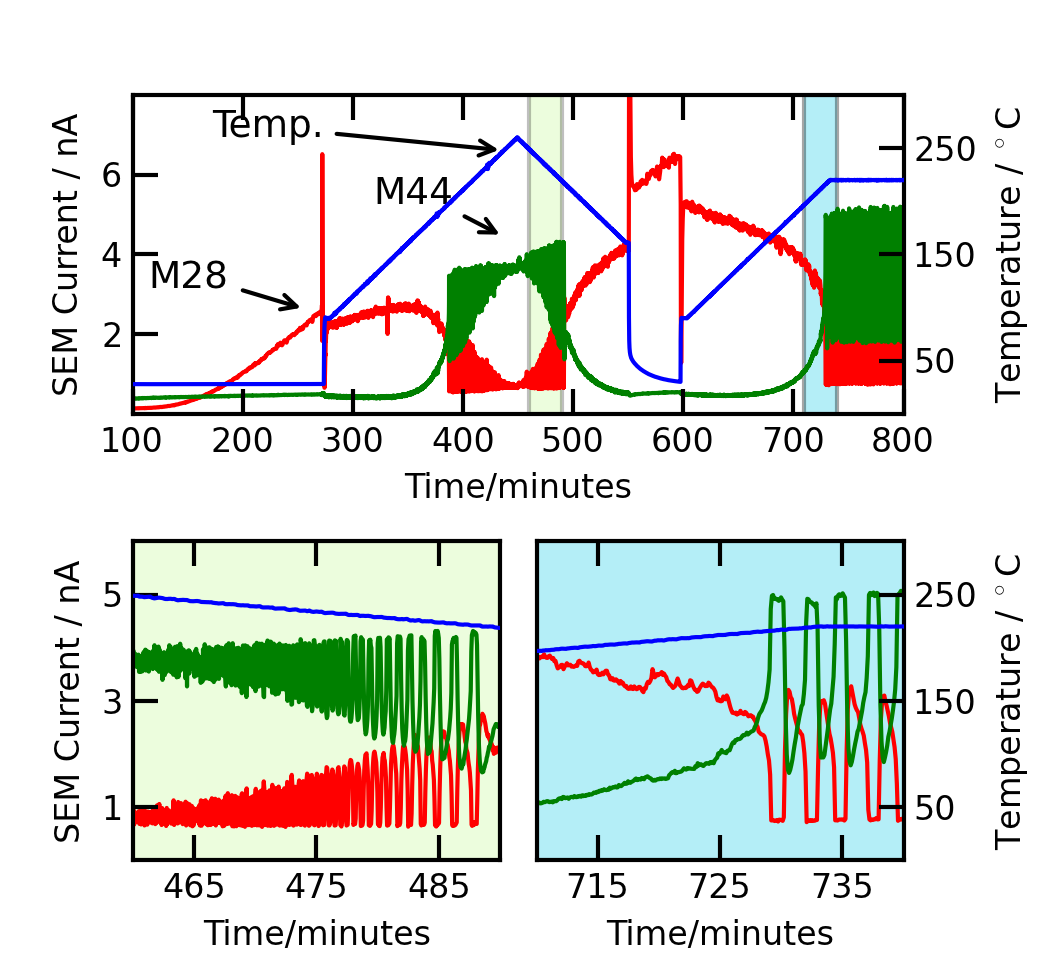
\includegraphics[width=9cm]{initial_treatment.png}
  \caption{A typical example of the initial treatment of a new sample. After performing a light-off ramp where oscillations can been seen the temperature is increased to a constant value where sustained oscillations take place. The non-zero value of CO during high conversion periods is consistent with the expected QMS background signals from CO$_2$ and O$_2$.}
  \label{fgr:initial_treatment}
\end{figure}
Nanoparticles with sizes ranging from 3\,nm to 9\,nm have been tested but 3\,nm particles with a geometrical coverage of 0.1\% of the reactor area gave the most stable oscillations. No consistent dependency on oscillation frequency and duty cycle was found that could be attributed to the size of the particles.

The oscillations on all samples are qualitatively similar but the oscillation period varies from a few seconds (the time-constant of the reactor is $\sim7\,$s) up to more than an hour. Once a sample start to oscillate consistently it will perform self-sustained oscillations for as long as the experiment is allowed to run. We have not observed a single sample stop oscillating once the self-sustained oscillations had started. 

An example of a single very slow oscillation is seen in Figure~\ref{fgr:full_oscillation}. After a short on-cycle (at $\sim$1030\,min.) where all CO is converted to CO$_2$ the reaction shows a fast deactivation. After the deactivation the sample quickly regains $\sim$30\% conversion (at $\sim$1040\,min.). Hereafter the conversion increases slowly over time until approximately 50\% conversion is reached (at $\sim$1118\,min.). Shortly after reaching 50\% conversion the sample again ignites and convert all CO to CO$_2$. After a short full conversion period the sample again deactivates and the cycle repeats itself.
\begin{figure*}
  \centering
  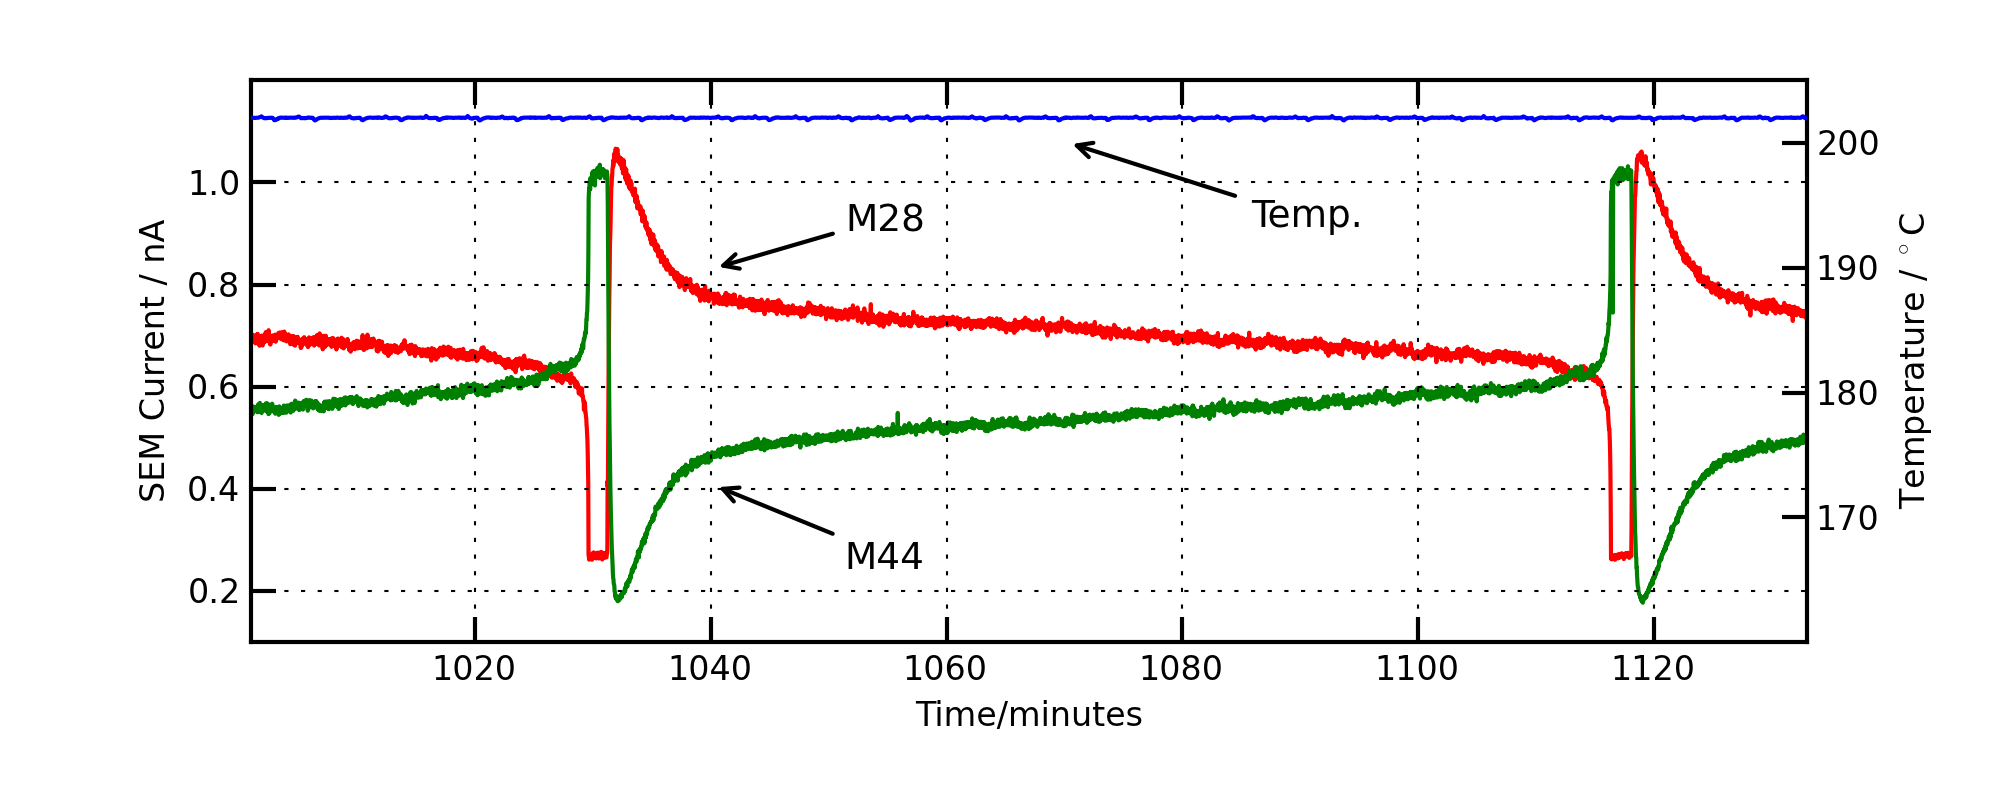
\includegraphics[width=17cm]{single_full_oscillation.png}
  \caption{A full oscillation period first showing a steep ignition of the sample followed by an almost immediate deactivation. For the next 65 minutes the sample slowly recovers activity until full conversion is reached again and the cycle repeats itself. This extremely long oscillation period is not commonly seen and was a result of careful parameter tuning. Typical oscillation periods are normally between $\sim$30\,s and $\sim$30\,minutes. Inserted circles illustrates the proposed model. At high conversion the platinum is oxidized (red) while in low conversion the sample is reduced (blue).}
  \label{fgr:full_oscillation}
\end{figure*}

After prolonged measurements over several days an increase in oscillation period was observed as shown in Figure \ref{fgr:long_measurement}. Initially, the oscillation period is $\sim$2.5 minutes and increases linearly with time until 1500 minutes of total oscillation time. Hereafter the oscillations become more irregular as shown in Figure~\ref{fgr:long_measurement}. At experiment end the oscillation period is between 45 and 20 minutes.
\begin{figure}[h]
\centering
  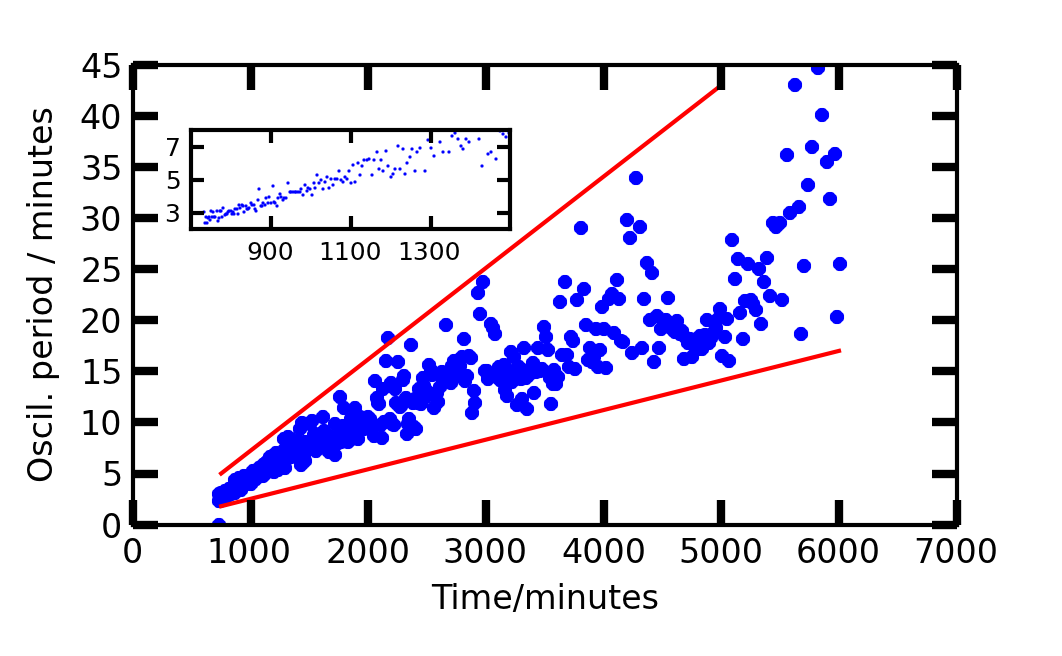
\includegraphics[width=9cm]{summary_of_long_measurement.png}
  \caption{Summary of the oscillation period as a function of time for a sample oscillating under constant temperature, pressure and reactant composition. The sample went through a total of 439 oscillations in 4 days. Time is defined from experiment start and hence includes initial treatment. The inset shows the initial steady increase in oscillation period.}
  \label{fgr:long_measurement}
\end{figure}
  
Figure~\ref{fgr:extracts} shows extracts of mass spectrometry data of oscillations extracted from the same four days measurement. Data from shortly after the initial treatment, after 2800\,min. of oscillation time and after 5900\,min are shown. After 5900\,min the oscillations are more irregular which is consistent with the data shown in Figure \ref{fgr:long_measurement}. Also, oscillations in between full conversion oscillations with smaller amplitude and much higher frequency than the full on-off cycles become more visible as time progresses.
\begin{figure}[h]
  \centering
  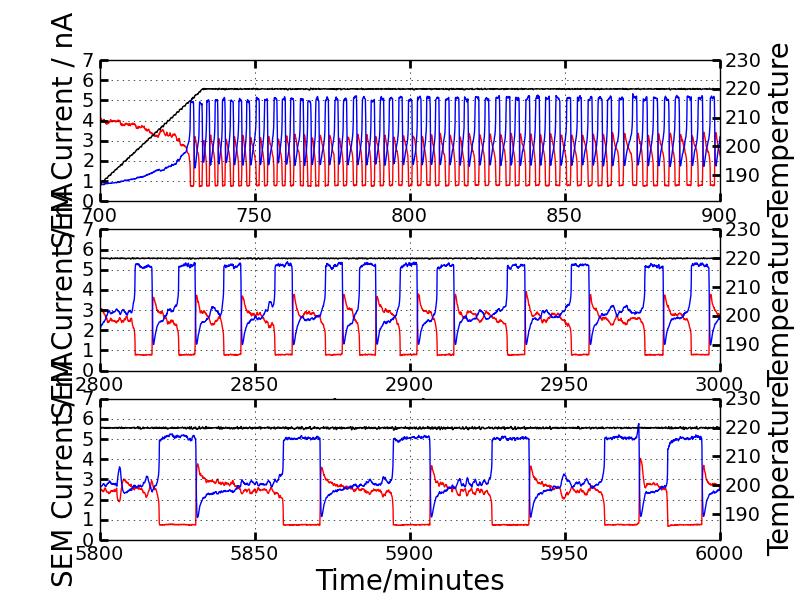
\includegraphics[width=9cm]{extracts_from_very_long_oscillation.png}
  \caption{Extracts from the 4 days long experiment. The oscillation period becomes more irregular with time while the total integrated conversion remains constant. Furthermore, small oscillations in between full conversion cycles become more prominent as time progresses.}
  \label{fgr:extracts}
\end{figure}

The oscillation frequency becomes more irregular with progressing experiment time as shown in Figure \ref{fgr:extracts}. However, the ratio between CO and CO$_2$ integrated over an full period remains constant throughout the entire experiment time, i.e. the samples maintains a constant average rate independent of oscillation frequency. 

%Furthermore, the oscillations have the qualitatively identical behavior as shown in Figure~\ref{fgr:full_oscillation}. A short full conversion period is followed by a fast deactivation from where reactivity is slowly recovered. At approximately 50\% conversion light-off occurs and the sample is in full conversion.

\begin{figure}[h]
\centering
  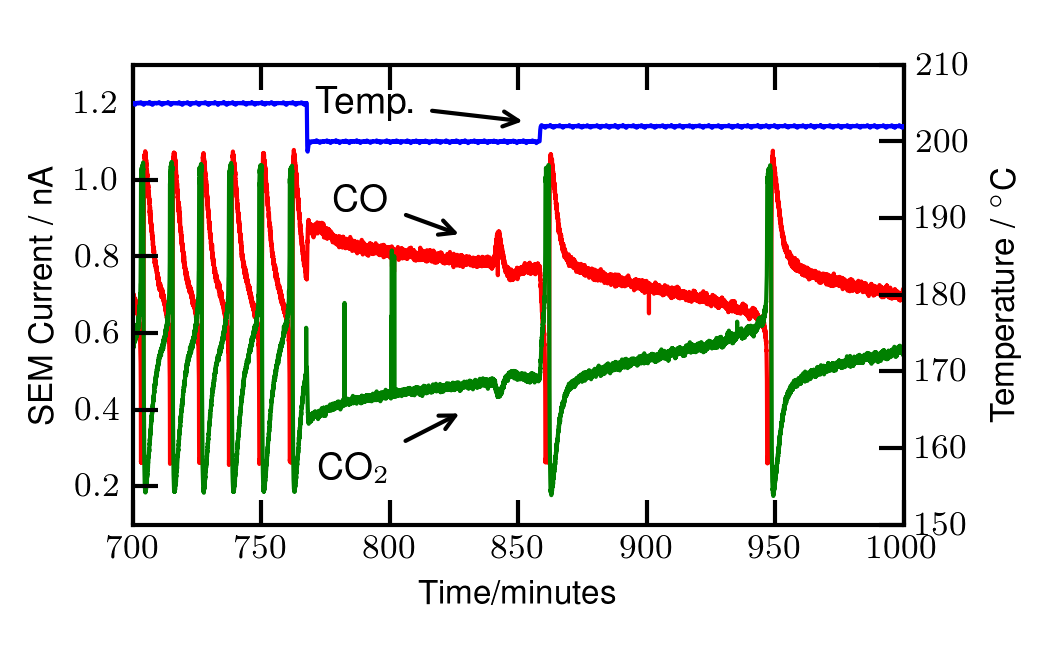
\includegraphics[width=9cm]{temperature_dependence.png}
  \caption{After about 10 hours of oscillations at 205$^\circ$C the temperature is first lowered by 5$^\circ$C and soon after increased by 2$^\circ$C. Before the temperature step the oscillation period was approximately 500\,s and after the step the period is approximately 5000\,s.}
  \label{fgr:temperature_dependence}
\end{figure}
A very strong temperature dependence on the oscillation frequency was also found as shown in Figure~\ref{fgr:temperature_dependence}. By changing the temperature 5$^\circ$C the oscillation period was changed by more than a factor of 10. The magnitude of the change is not completely consistent across all measured samples but all samples show a very large temperature dependency where in some cases a provoked small change in temperature will consistently turn on and off the oscillations.

The pressure dependence of the oscillations was also investigated. In the pressure range of 0.1\,bar to 1\,bar no change of the oscillation frequency or qualitative behavior that could be attributed to the pressure was found. Similarly, only a weak dependence on the CO/O$_2$ ratio was observed. At a CO/O$_2$ ratio of $\sim0.025$ only very small amplitude oscillations was observed. Increasing the CO/O$_2$ showed clear oscillations with a significant increase in oscillation amplitude compared to lower CO concentrations. Generally, a tendency towards longer oscillation periods for higher CO/O$_2$ ratio was observed. Richer CO mixtures than 0.175 did not produce any oscillations in our system.

Although oscillations have previously been observed on extended Pt thin films \cite{Singh2010} as well as single crystals\cite{Hendriksen2005} at atmospheric pressure no oscillations could be provoked on thin films of comparable geometrical coverage to the nanoparticles in our system at any CO/O$_2$ ratio.  

%No consistent dependency on oscillation frequency and duty cycle was found that could be attributed to the size of the particles.

\section{Discussion}
Due to the long timescales between full conversion and low conversion plateaus the oscillations cannot be attributed to the reactor setup itself which due to its small size has timescales on the order of seconds. Furthermore, a series of experiments was performed to exclude the oscillations as an instrumental artifact. Firstly, experiments were performed on larger volume reactor thus increasing the residence time in the reactor. Secondly, the oscillations were reproduced on a comparable but not identical setup. Finally, attempts at reproducing the phenomenon on Pt-thin films of comparable coverage did not produce any oscillations. All of these experiments suggest that the oscillations is a property of the Pt nanoparticles.

It has previously been shown using STM \cite{Hendriksen2002}, FT-IR \cite{Carlsson2006}, Monte Carlo simulations \cite{Zhdanov2002} as well as DFT \cite{Gong2004} that the activity of Pt towards CO oxidation at atmospheric pressures is highly dependent on the oxidation state of the surface. A detailed proposal for the reaction mechanism on Pd has been developed by Hendriksen \textit{et. al.}\cite{Hendriksen2010} and our data is consistent with this model.

According to the proposed model in ref.~\citenum{Hendriksen2010} the bare metal surface is less active than the oxidized surface. Oscillations originate from a switch between an oxidized surface and the bare metal surface. Initially, with CO present in the inlet gas a smooth metal surface is exposed due to the general high adsorption energy of CO on metal surfaces. As the Pt nanoparticles convert the CO to CO$_2$ the partial pressure of CO will decrease and a Pt oxide will start to form in the high partial pressures of O$_2$ thus increasing the rate. The model\cite{Hendriksen2010} suggests that the oxidized nanoparticles will roughen during CO oxidation resulting in the formation of an increasingly rough oxide surface. As the oxide becomes rougher the bare metal surface is increasingly favored resulting in a return to the lower rate rough metal state. As the rate decreases the CO partial pressure increases which results in a transition from rough metal surface to a smooth metal surface. When the sample is sufficiently smooth it will again oxidize and thus complete the oscillation cycle. 

In this study Pt nanoparticles were investigated which, compared to a single crystal or a thin film, is a very rough surface. It is to be expected that the particles will initially favor the reduced state. As the reaction runs the gas composition towards the outlet of the reactor will become more oxidizing increasing the oxidation rate of the particles (illustrated in Figure~\ref{fgr:full_oscillation}). Gradually, as the particles toward the outlet oxidizes the turn-over will increase and the general CO concentration will decrease promoting more and more particles to oxidize which will gradually be seen in the QMS as an increase in CO$_2$ and a decrease in CO. As the CO concentration decreases the light-off temperature will decrease hence approaching the constant temperature of the sample resulting in a steep increase in reactivity. It is important to note that the fraction of oxidized particles needed to achieve full conversion is not known. We are currently investigating new methods for gaining insight into the nature of the nanoparticles in the reactor but the low coverage and the design of the reactor makes this a challenging task. If not all particles are oxidized at light-off they will now oxidize much faster due to the low CO-concentration. The further increased rate will not be visible in the QMS since the reactor is already in full conversion. As most of the particles are now oxidized they will become more and more roughened and gradually return to the reduced state. Fewer and fewer oxidized particles will be responsible for the activity increasing the roughing rate of the remaining active particles. Just before the overall activity drops only a fraction of the particles participates in the reaction and the deactivation will happen very suddenly. Once these potentially few particles eventually becomes sufficiently rough they will reduce and lose activity hence completing the oscillation cycle. It should be noted that our group has recently measured turnover frequencies of CO oxidation on Pt in excess of $10^{6}$s$^{-1}$ per site corresponding to as little as $\sim$300 Pt nanoparticles contributing to the reactivity just before the end of the high-activity cycle.

The oscillation period increases with time and becomes increasingly less stable as shown in Figure~\ref{fgr:extracts}. This phenomena is consistent across all measured samples. The large scatter in oscillation period can be attributed to the smaller oscillations in between on/off cycles. Occasionally, these small amplitude oscillations will trigger a full switch thus introducing more short-period oscillations despite the trend of increasingly slower oscillation period. This could suggest either sintering or roughening of the clusters. However, since the average conversion integrated over full oscillation periods is constant we do not expect sintering to be the cause where an average loss in activity of the sample would be expected.

Oscillations were only seen in CO/O$_2$ ratio below 0.175. This ratio agrees well with literature \cite{Singh2010,Hendriksen2005} where oscillations have been observed in oxygen rich CO/O$_2$ mixtures. The needed low concentration of CO in the inlet gases can be attributed to the much higher sticking coefficient of CO on Pt which poisons the nanoparticle surface during the low reactivity region of the cycle. 

Nanoparticles of several different sizes were tested and all showed oscillations. However, no change in duty cycle or frequency that could be attributed to the size of the nanoparticles was found. This may be due to the fact that even nominally identical samples also show a large variation in oscillation frequency and duty cycle thus possibly shadowing a nanoparticle size effect.

An interesting feature in the data is the very large temperature dependence on oscillation frequency. This property agrees well an earlier suggested model \cite{Hendriksen2010} and it is, to our knowledge, the first time the temperature dependence of oscillations at atmospheric pressure has been measured.

\section{Conclusion}
Self-sustained CO oxidation oscillations at atmospheric pressure on Pt nanoparticles ranging from from 3\,nm to 9\,nm have been measured with high-quality mass-spectrometry. It was found that the samples increased the oscillation period over time and showed a strong temperature dependence. A model is proposed where the nanoparticles go through repetitive oxidation/reduction cycles which change the change rate of CO oxidation on the particles.

%\subsection{This is the subsection heading style}
%Section headings can be typeset with and without numbers.\cite{Gong2004} \cite{Hendriksen2010}

%\subsubsection{This is the subsubsection style.~~} These headings should end in a full point.  

%\paragraph{This is the next level heading.~~} For this level please use \texttt{\textbackslash paragraph}. These headings should also end in a full point.

%\section{Equations}

%Equations can be typeset inline \textit{e.g.} $ y = mx + c$ or displayed with and without numbers:

% \[ A = \pi r^2 \]

%\begin{equation}
%  \frac{\mathrm{\gamma}}{\mathrm{\epsilon}x} r^2 = 2r
%\end{equation}

%\section{Graphics and tables}
%\subsection{Graphics}
%Graphics should be inserted on the page where they are first mentioned (unless they are equations, which appear in the flow of the text).



%\subsection{Tables}
%Tables typeset in RSC house style do not include vertical lines. Table footnote symbols are lower-case italic letters and are typeset at the bottom of the table. Table captions do not end in a full point.


%\begin{table}[h]
%\small
%  \caption{\ An example of a caption to accompany a table}
%  \label{tbl:example}
%  \begin{tabular*}{0.5\textwidth}{@{\extracolsep{\fill}}lll}
%    \hline
%    Header one/units & Header two & Header three \\
%    \hline
%    1 & 2 & 3 \\
%    4 & 5 & 6 \\
%    7 & 8 & 9 \\
%    10 & 11 & 12 \\
%    \hline
%  \end{tabular*}
%\end{table}

%Adding notes to tables can be complicated.  Perhaps the easiest
%method is to generate these manually.

% an example of a two-column table
%\begin{table*}
%\small
  %\caption{\ An example of a caption to accompany a table, table captions do not end in a full point}
  %\label{tbl:example}
  %\begin{tabular*}{\textwidth}{@{\extracolsep{\fill}}lllllll}
    %\hline
    %Header one & Header two & Header three & Header four & Header five & Header six  & Header seven\\
    %\hline
    %1 & 2 & 3 & 4 & 5 & 6  & 7\\
    %8 & 9 & 10 & 11 & 12 & 13 & 14 \\
    %15 & 16 & 17 & 18 & 19 & 20 & 21\\
    %\hline
  %\end{tabular*}
%\end{table*}

%You can also put lists into the text. You can have bulleted or numbered lists of almost any kind. 
%The \texttt{mhchem} package can also be used so
%that formulae are easy to input: \texttt{\textbackslash ce\{H2SO4\}} gives \ce{H2SO4}. 


%\section{Conclusions}
%The conclusions section should come at the end of article. For the reference section, the style file rsc.bst can be used to generate the correct reference style.\footnote[4]{Footnotes should appear here. These might include comments relevant to but not central to the matter under discussion, limited experimental and spectral data, and crystallographic data.}
 %For footnotes in the main text of the article please number the footnotes to avoid duplicate symbols. e.g.  \footnote[num]{your text} the corresponding author \ast counts as footnote 1, ESI as footnote 2, e.g. if there is no ESI, please start at [num]=[2], if ESI is cited in the title please start at [num]=[3] etc. Please also cite the ESI within the main body of the text using \dag.





%The \balance command can be used to balance the columns on the final page if desired. It should be placed anywhere within the first column of the last page.

%\balance

%If notes are included in your references you can change the title from 'References' to 'Notes and references' using the following command:
%\renewcommand\refname{Notes and references}

\footnotesize{
\bibliography{literature} %your .bib file
\bibliographystyle{rsc} %the RSC's .bst file
}

\end{document}
